The system architecture is divided in 5 tiers and it's implemented using then Java Enterprise Edition framework.
\begin{itemize}
    \item The first tier is the client tier: it contains the mobile application running on customers' devices and the web browser used by the store employees and the store manager to access the web application of CLup. The former communicates with the JEE server via a REST interface. The latter accesses the web server and retrieves web pages.
    \item The second tier is the web tier: it is composed of the web server implemented with the Apache HTTP platform. It mainly serves the static content and it is connected with the Tomcat script server to load the dynamic data.
    \item The third tier contains the script engine server. Tomcat has been choosed as the platform to generate dynamic content, via Servlet or JSP, requested by the Apache HTTP server.
    \item The fourth tier is the application logic tier: it is composed of the WildFly application server platform which handles the Enterprise Java Beans to which the Tomcat server connects.
    \item On the data tier (tier 5) there is the Database server. The connection with the tier 4 is implemented with a JDBC connector.
\end{itemize}

\begin{figure}[H]
    \centering
    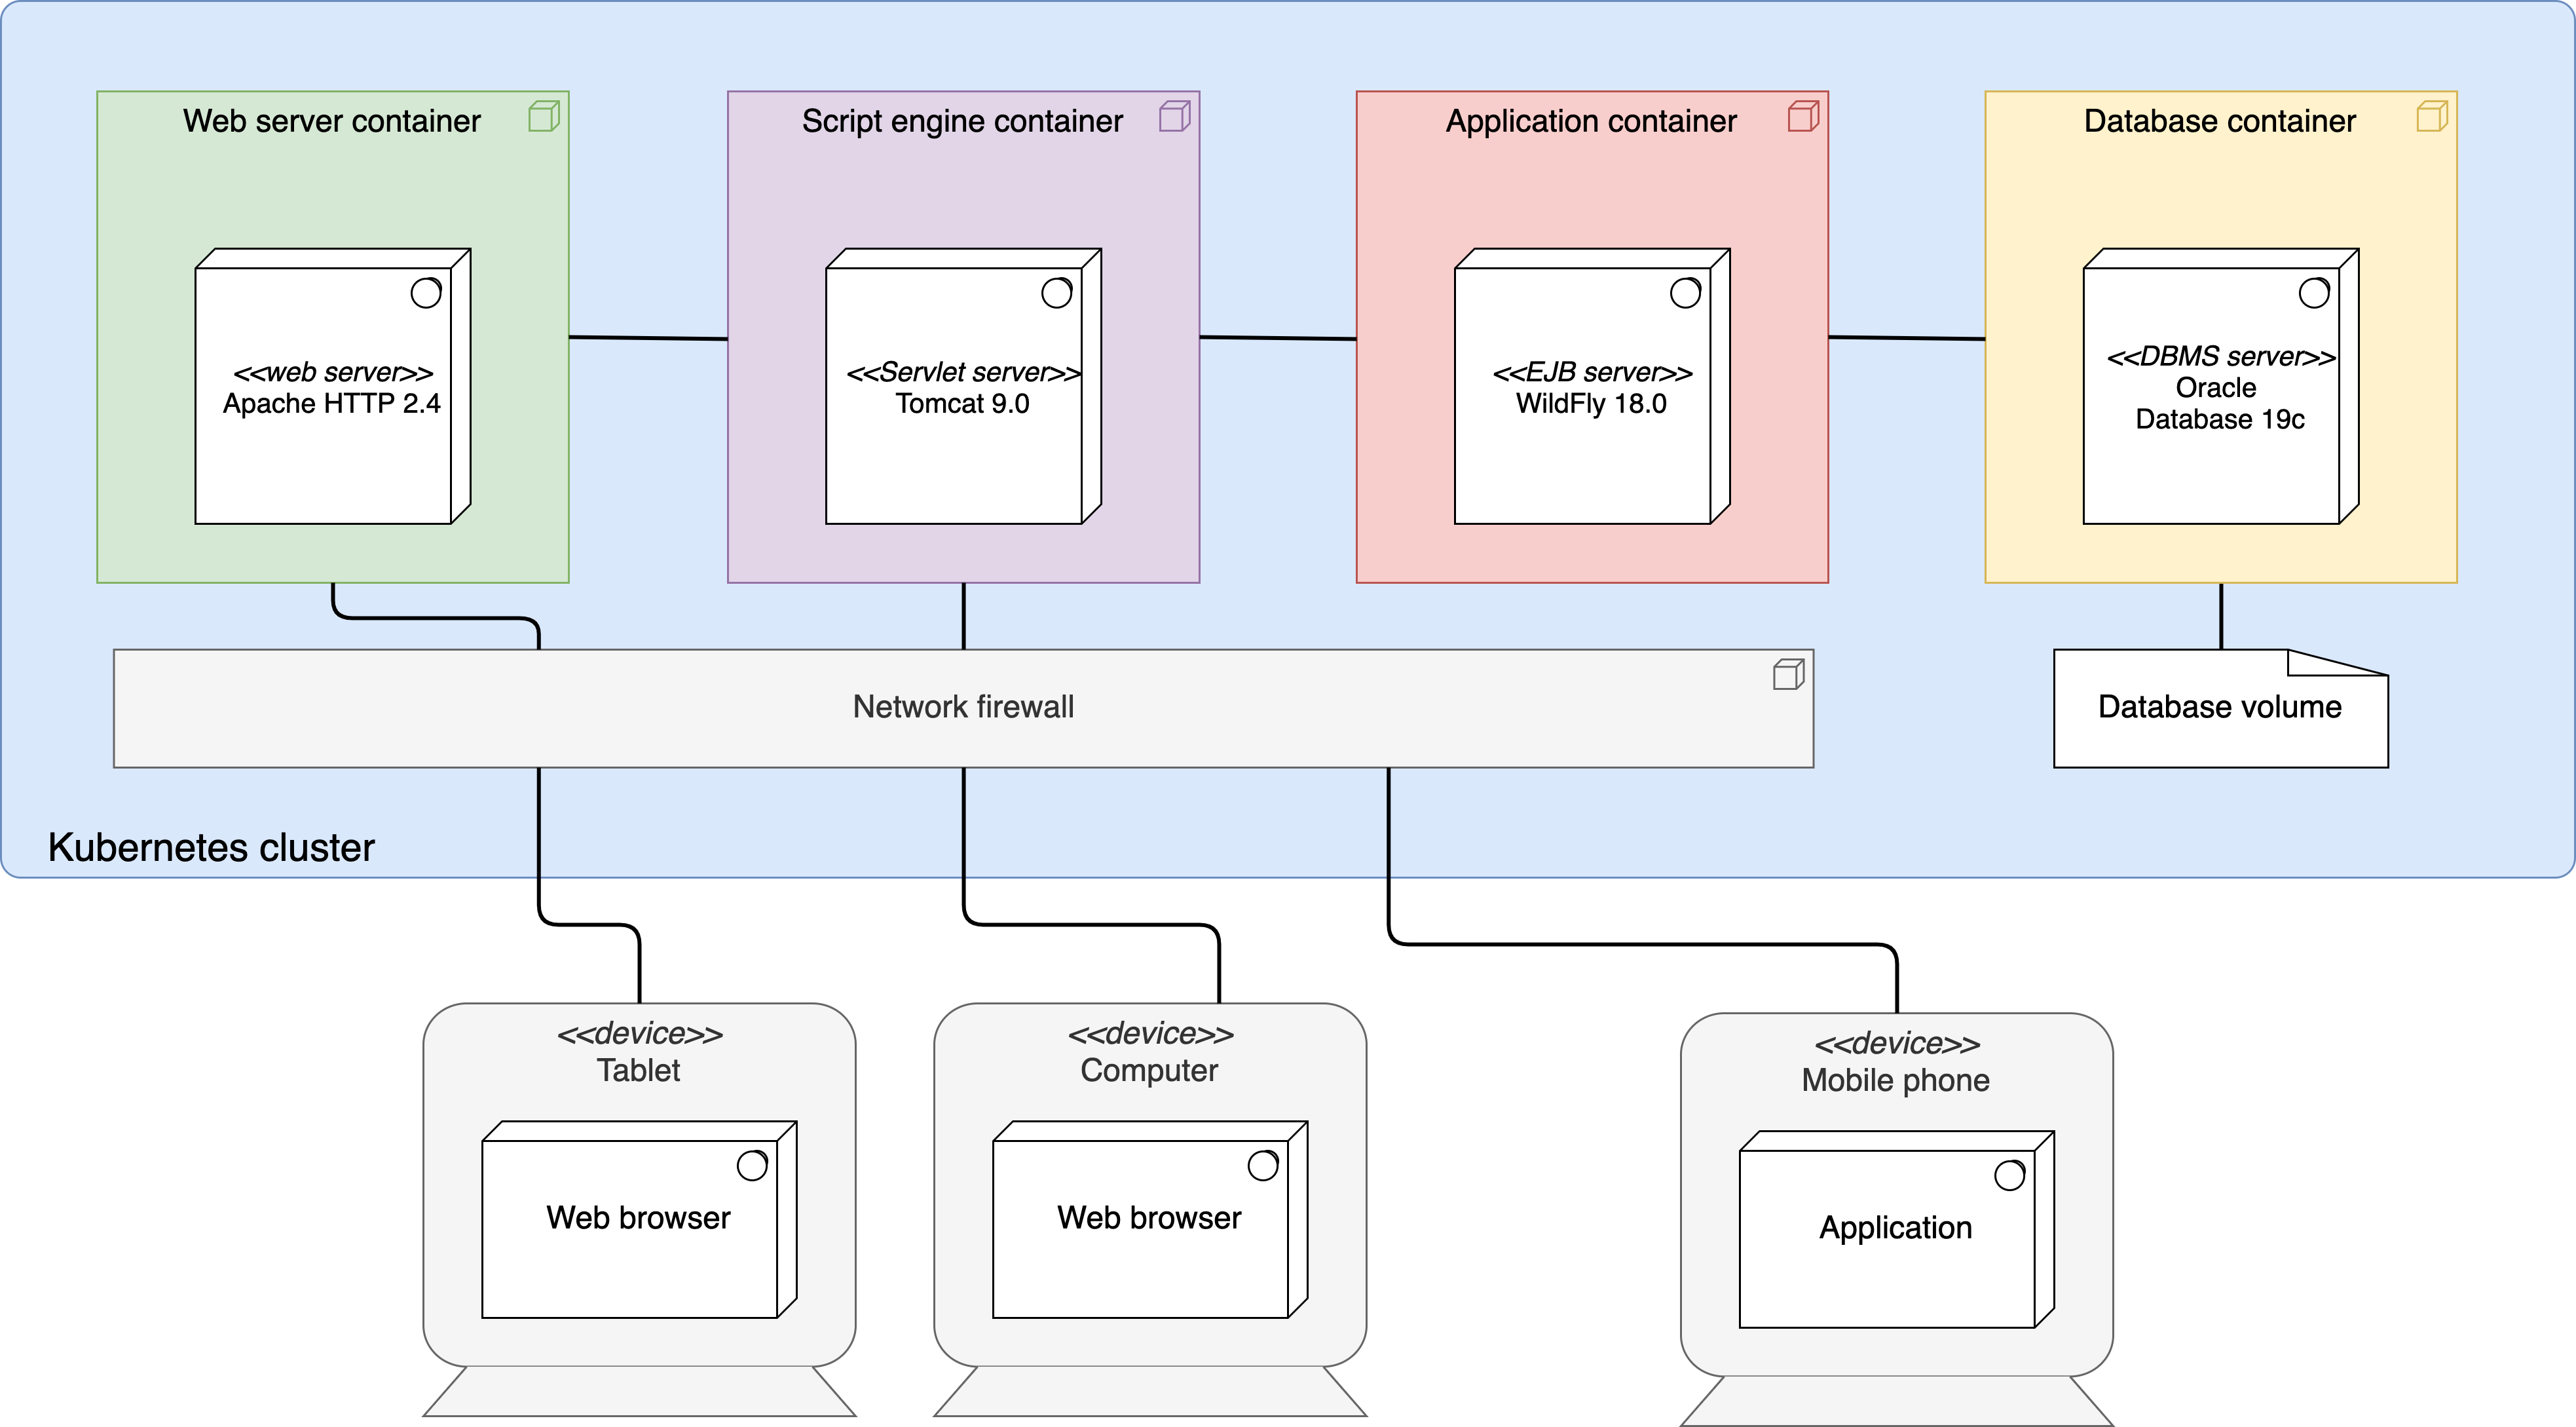
\includegraphics[width=16cm]{deployment_view.png}
    \caption{Deployment diagram}
\end{figure} 

\textbf{Recommended deployment:}

All the tiers, except the first one, may be deployed as containers in a Kubernetes cluster. Each of the four tiers may be containerized and then deployed in a cluster. This process would produce many advantages such as:
\begin{itemize}
    \item Easy replication management: it as easy as to change a number in a configuration file to scale up or down one of the tiers (except for the database, which is a little bit more involved).
    \item Portability: the application is extremely portable between different physical or cloud deployments, for example, allowing to switch between geographically different datacenters in a couple of minutes.
    \item Easy update management: update release is only a matter of shutting down some containers and bringing up new ones from updated images. Moreover, different versions of the system can coexist at the same time on the same cluster.
\end{itemize}
The Kubernetes cluster may be created and managed by the CLup deployment team. A better option may be to directly deploy the containers to Amazon EKS, Google Kubernetes Engine, or similar cloud services. In the latter case, tier 5 may use a service like Amazon EFS or Google Firestore to store the database, allowing to make copies of the database and protect against hard failures with an automatic backup solution offered by those cloud providers.

\bigbreak
\textbf{Recommended implementation:}
\begin{itemize}
    \item \textbf{Client tier:} the customer mobile application may be implemented using a cross platform development framework like Flutter. Flutter allows to write the application code once and then to easily compile the source code for both Android and iOS systems. This would be a big advantage in terms of reducing development cost and time and of obtaining code maintainability. 
    \item \textbf{Web tier:} the web pages of the web application may be implemented with HTML 5.0, CSS and JavaScript. 
    \item \textbf{Script engine tier:} the dynamic content may be generated using Java Servlets
    \item \textbf{Application logic tier:} the EJB application server may use stateless Java Beans connected using JPA with the Database server. This would allow having the client state completely stored on the DBMS, thus allowing to easily scale up or down the business instances.
    \item \textbf{Data tier:} the database may be implemented with MySQL Server Enterprise Edition.
\end{itemize}